\documentclass[a4paper, 10pt,onecolumn]{scrartcl}

%Standardpakete Deutsch
\usepackage[ngerman]{babel}
\usepackage[T1]{fontenc}
\usepackage[utf8]{inputenc}

%Extras
\usepackage{multirow}
\usepackage{natbib}
\usepackage{graphicx}
\usepackage{amsmath, amssymb}
\usepackage{graphicx}
\usepackage{grffile} %einfacheres einbinden von Dateipfaden
\usepackage{xpatch} %more space between title and subtitle
\usepackage{mathtools}
\usepackage{booktabs}
\newcommand{\changefont}[3]{
\fontfamily{#1} \fontseries{#2} \fontshape{#3} \selectfont}
\usepackage[export]{adjustbox}

\newlength{\myspace}
\setlength{\myspace}{2em}

\makeatletter
\xpatchcmd{\@maketitle}{\vskip.5em}{\vskip\myspace}{}{}
\makeatother

%\changefont{ptm}{m}{n}

\title{Computational Physics 1: Übung 6: Fouriertransformation} 
\author{Jakob Hollweck} %auch nach \begindocument möglich
\setlength{\parindent}{0pt}
\date{Abgabe 12.01.18}

\begin{document}
\maketitle


\section*{Aufgabe 1: Sampling einer Schwebung}

Das in Abbildung \ref{Abbildung1} zu sehende Frequenzspektrum wurde mithilfe einer Fast-Fourier-Transformation (FFT) der Schwebung $S(t) = \sin(5t) + \sin(\omega t)$ für $\omega \in \{1,2,...,14,15\}$, die für $N=256$ und $t \in [0,30\pi]$ abgetastet wurde, berechnet.


\begin{figure}[ht!]
	\centering
	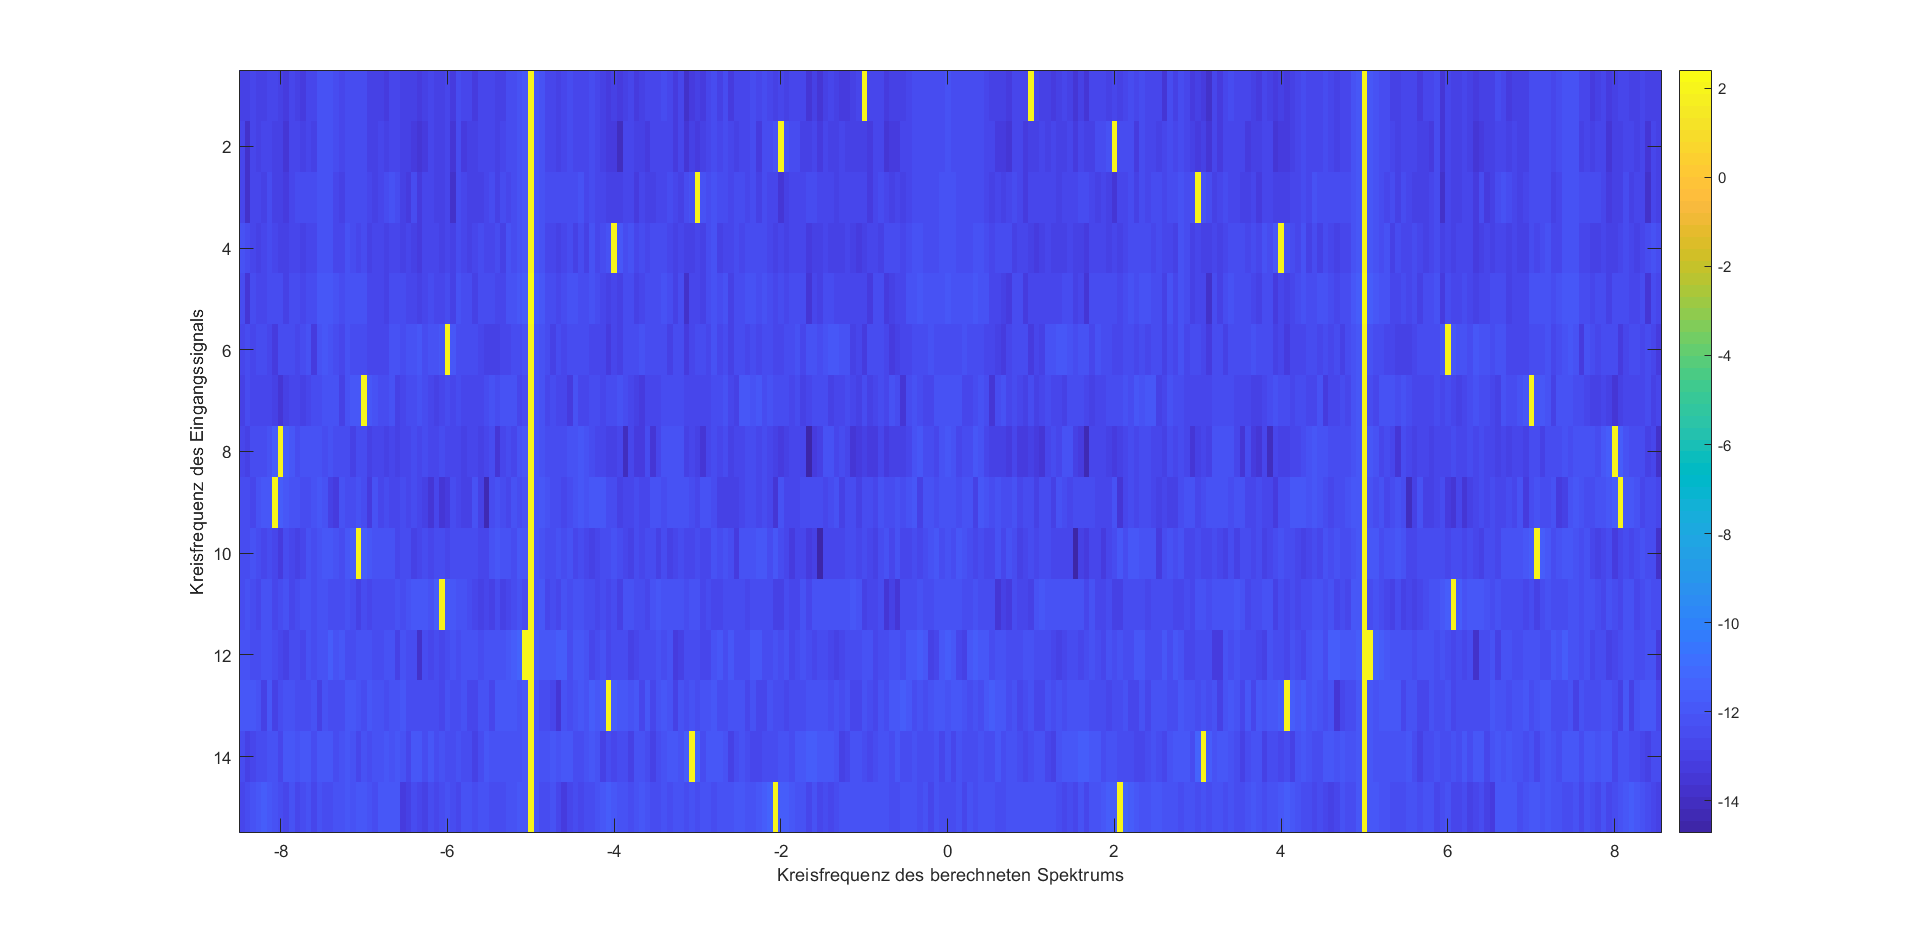
\includegraphics[scale=0.4,center]{sem06_1_3.png}
	\caption{Fourierspektren der Schwebung $S(t)$ für verschiedene $\omega$} 
	\label{Abbildung1}
\end{figure}

Die durchgeführte FFT berechnet die beiden Kreisfrequenzen $\omega$ von $S(t)$, wobei $\omega = 5$ konstant gehalten wird. Dies ist gut am Spektrum durch die beiden Linien bei $\omega = 5$ und $\omega = -5$ zu erkennen.
Während der Berechnung wird der Betrag der einzelnen Komponenten des Spektrums gebildet, was eine Symmetrie bezüglich $\omega = 0$ verursacht.
Des weiteren zeigt das Spektrum, dass die FFT für $\omega \leq 8$ eine korrekte Kreisfrequenz ausgibt, für höhere Eingangsfrequenzen sinkt die berechnete Kreisfrequenz dagegen fälschlicherweise.
Der Grund hierfür liegt im Abtasttheorem, die eine höchste Frequenz $\nu_{max}$ für die Beschreibung im Fourierraum vorgibt. Nach diesem gilt: 

\begin{equation}
	\nu_{max} \leq \frac{1}{2}\ \nu_{abtast}
\end{equation}

Diese ergibt sich hier zu $\nu_{max} = \frac{1}{2} \frac{256}{30\pi} \approx 1,36$ bzw. $\omega_{max} \approx 8.53$, was sich ungefähr in Abbildung \ref{Abbildung1} erkennen lässt. Durch eine zu langsame Abtastung werden Extrema des Signals verpasst, was dieses mit niedrigerer Frequenz erscheinen lässt.
\newpage

\section*{Aufgabe 2: Scheinbare Verbesserung der Auflösung durch Einfügen von Nullsignalen}

Im zweiten Aufgabenteil wurde das Verhalten der FFT bei Hinzufügen von Nullsignalen im Funktionswerte untersucht. Dafür wurde ein Gaußsignal $G(t) = \exp(-2(t-\pi)^2)$ mit 16 Stützstellen im Intervall $[0,2\pi]$ abgetastet und zum Vergleich dem selben Signal $2^n$ Nullen, für $n \in \{4,5,6,7,8,9\}$, angefügt, um Abtastraten von 16 bis 512 zu erhalten. Das Ergebnis ist in Abbildung \ref{Abbildung2} zu sehen. 


\begin{figure}[ht!]
	%\centering
	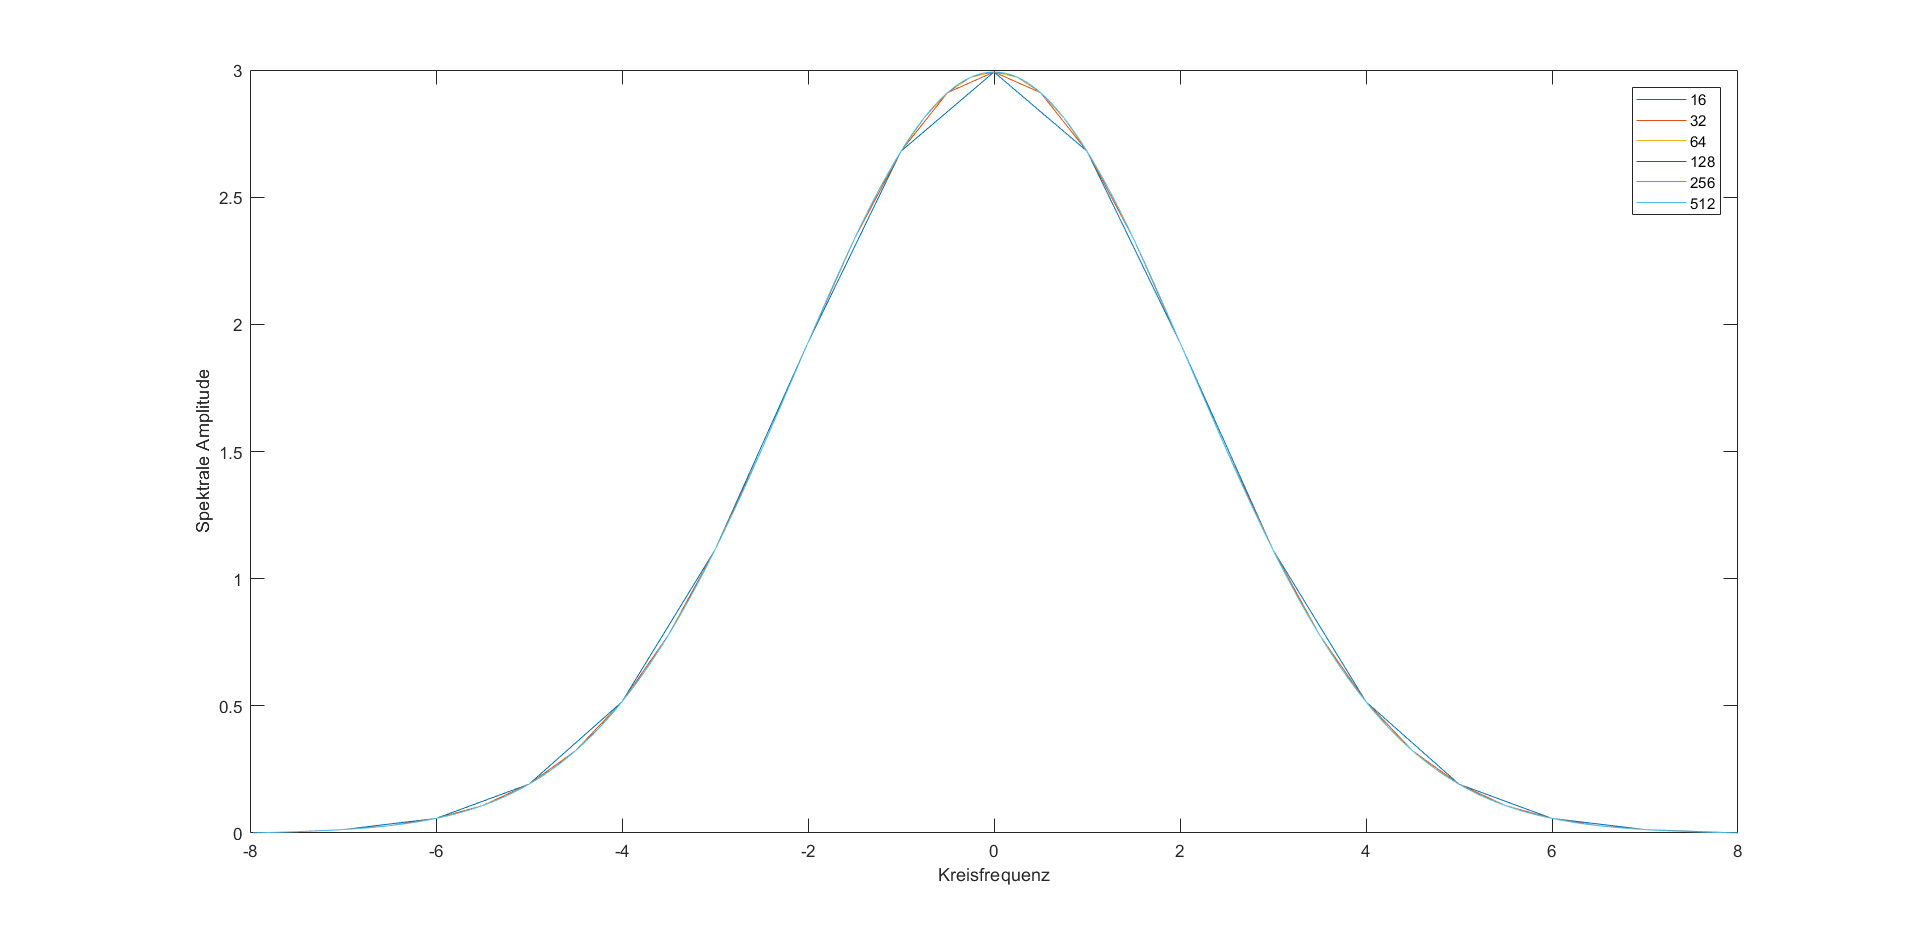
\includegraphics[scale=0.4,center]{sem06_2_2.png}
	\caption{Fouriertransformation des Gaußpulses $G(t)$, abgetastet mit 16 Stützstellen im Intervall $[0,2\pi]$. Die weiteren Graphen mit scheinbar mehr Stützstellen wurden durch das Anfügen von Nullen im Funktionswert erzeugt.  } 
	\label{Abbildung2}
\end{figure}


Das Frequenzspektrum formt für höhere Abtastraten ein schärferes Maximum aus, da durch das vergrößern der Bandbreite die Frequenzauflösung steigt. Die Auflösung ist natürlich nur dann verbessert, wenn das Signal im erweiterten Bereich auch wirklich auf 0 abgefallen ist.  

\end{document}